% $Id$
%
% Copyright (C) 2019 by GONG Jie <gongjie.jie@gmail.com>
%
% Permission to use, copy, modify, and/or distribute this software for any
% purpose with or without fee is hereby granted.
%
% THE SOFTWARE IS PROVIDED "AS IS" AND THE AUTHOR DISCLAIMS ALL WARRANTIES
% WITH REGARD TO THIS SOFTWARE INCLUDING ALL IMPLIED WARRANTIES OF
% MERCHANTABILITY AND FITNESS. IN NO EVENT SHALL THE AUTHOR BE LIABLE FOR ANY
% SPECIAL, DIRECT, INDIRECT, OR CONSEQUENTIAL DAMAGES OR ANY DAMAGES
% WHATSOEVER RESULTING FROM LOSS OF USE, DATA OR PROFITS, WHETHER IN AN ACTION
% OF CONTRACT, NEGLIGENCE OR OTHER TORTIOUS ACTION, ARISING OUT OF OR IN
% CONNECTION WITH THE USE OR PERFORMANCE OF THIS SOFTWARE.
%
\documentclass{cookbook}
\input{git-revision.tex}
\usepackage{hyperref}
	\hypersetup{
		bookmarks=true,
		unicode=true,
		pdfduplex={DuplexFlipLongEdge},
		pdfprintscaling={AppDefault},
		pdfpicktraybypdfsize={true},
		pdftoolbar={false},
		pdftitle={四川菜谱},
		pdfauthor={成都市饮食公司革命委员会技术培训班},
		pdfsubject={},
		pdfkeywords={},
		pdfcreator={},
		pdflang={zh-CN},
		pdfinfo={
			GitCommitHash={\gitcommithash},
			GitAuthorDate={\gitauthordate}
		},
		hidelinks
	}

\begin{document}
\begin{cookbook}

\pagestyle{empty}

\definecolor{pantone485}{cmyk}{0, 1, 1, 0}
\textcolor{pantone485}{%
	\null%
\vspace{1.5\baselineskip}
\sffamily%
\begin{center}
{%
	\huge\bfseries%
	{\hbadness=1500\makebox[5.6em][s]{毛主席語录}}
}
\end{center}

\begingroup%
\Large\bfseries%
\doublespacing%
\setlength{\parindent}{1.8em}%

路线是个纲,纲举目张。

全心全意地为人民服务。

发展经济,保障供给。

为什么人的问题,是一个根本的问题,\kern-.6em\\
\kern-.2em原则的问题。

\endgroup

% vim: filetype=tex noautoindent nojoinspaces
% vim: fileencoding=utf-8 formatoptions+=m
% vim: textwidth=78 tabstop=4 shiftwidth=4 softtabstop=4

}
\cleardoublepage

\null%
\vspace{.75\baselineskip}
\begin{center}
\begin{tabular}{r}
	{\Huge\bfseries \makebox[3.86em][s]{四川菜谱}}\\%
	{\normalsize\bfseries 1972\,\makebox[2.78em][s]{重制版}}%
\end{tabular}

\vfill

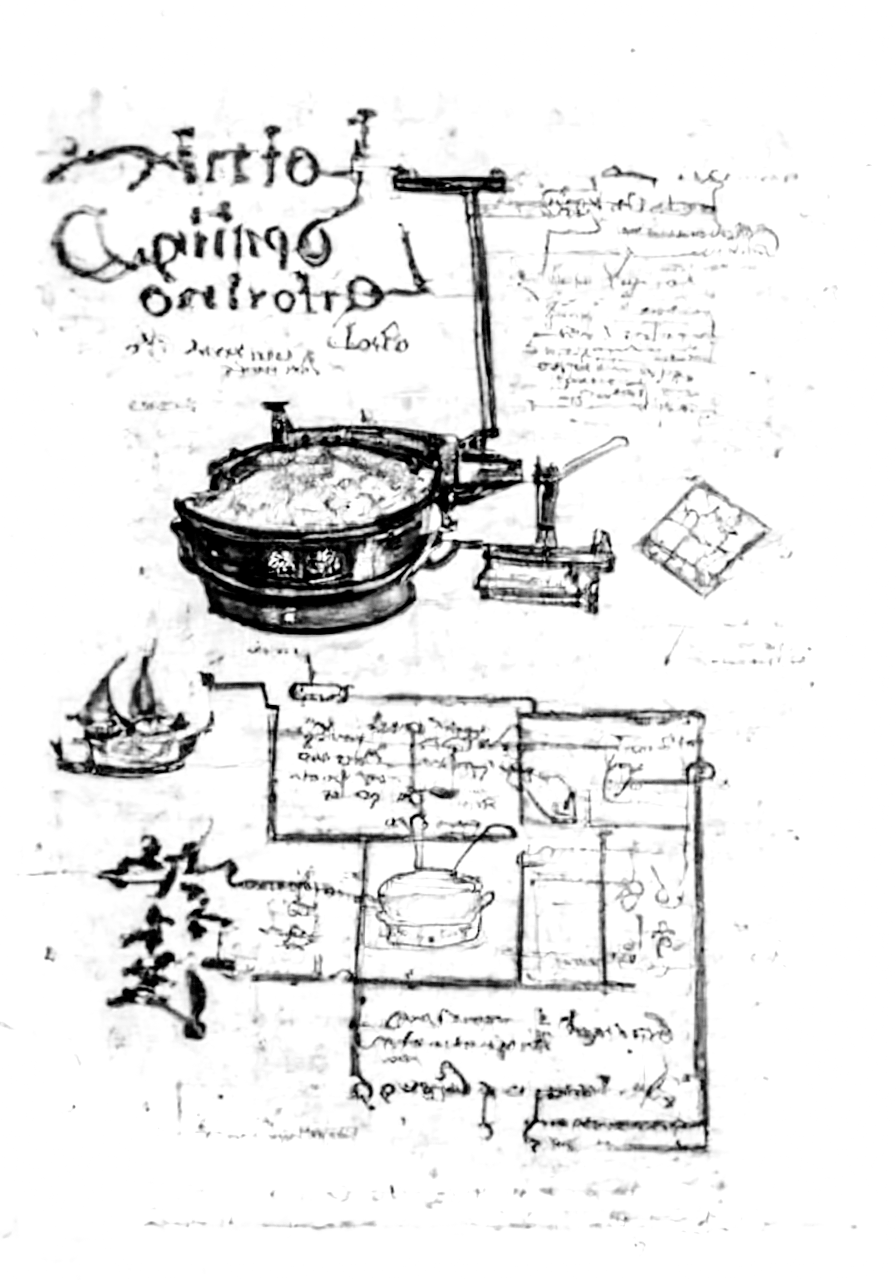
\includegraphics[height=118.070219mm]{cooking-machine.png}%

\vfill

{\footnotesize \textsc{Quux} System and Technology}
\end{center}

% vim: filetype=tex noautoindent nojoinspaces
% vim: fileencoding=utf-8 formatoptions+=m
% vim: textwidth=78 tabstop=4 shiftwidth=4 softtabstop=4

\cleardoublepage

\begin{center}
\Large
编印说明
\end{center}

在伟大领袖毛主席{\sffamily“发展经济,保障供给”}的财政经济工作总方针的指引下,商业战线同各条战线一样,形势大好,越来越好。我们饮食服务工作,为了适应革命、生产大好形势的不断发展,进一步继承和发扬祖国的烹调遗产,提高饮食部门的口味质量,增加花色品种,使饮食烹调技术更好地为广大工农兵服务,我们在有关部门的帮助和支持下,编印了这本《四川菜谱》。

在编写《四川菜谱》的过程中,我们参照了过去积累的资料,同时也结合我们在实际操作中初步摸索到的一些经验,特别是经过无产阶级文化大革命运动,遵照毛主席关于{\sffamily“我们必须继承一切优秀的文学艺术遗产,批判地吸收其中一切有益的东西”}的教导,对菜谱的品种、名称、内容等各个方面作了必要的修改整理并有所取舍。这次主要参照了过去我们编写的《中国名菜谱第七辑》和搜集《重庆名菜谱》部分菜肴,内容分肉食、鸡鸭、鱼虾、山珍海味、甜食、蔬菜、其它七个大类,共三百一十二个品种,基本上按由浅入深,由简到繁的次序编排。

《四川菜谱》作为内部资料编印,主要是作为我们培训技术的教材用的。由于我们的理论水平和技术水平都比较低,又缺少经验,这次编写《四川菜谱》一定会有不少缺点,希望广大饮食服务战线的同志们,特别是具有丰富实践经验的老师傅,给我们提出宝贵的意见,以便及时改进。为使饮食烹调技术更好地为广大工农兵服务而共同努力。

\begin{flushright}
成都市饮食公司革命委员会\\
技术培训班教研组集体整编

一九七二年七月
\end{flushright}

% vim: filetype=tex noautoindent
% vim: fileencoding=utf-8
% vim: textwidth=78 tabstop=4 shiftwidth=4 softtabstop=4

\cleardoublepage

\pagestyle{fancy}

\frontmatter

\tableofcontents

\mainmatter

\category{肉食类}
\begin{recipe}{回锅肉}

\ingredients

\ingredient{猪肉}{一斤三两}
\ingredient{甜红酱油}{三钱}
\ingredient{豆豉}{一钱}
\ingredient{豆瓣}{五钱}
\ingredient{蒜苗}{二两}
\ingredient{甜酱}{二钱}
\ingredient{化猪油}{六钱五}

\preparation

\step 选用二刀猪腿肉,洗净去毛,入汤锅内煮二十分钟,以煮至肉皮软时适宜;捞出稍
晾,切成一分厚、一寸二宽、一寸五长、肥瘦相连的片。豆瓣、豆豉均剁成细茸。蒜苗多
用蒜头部分,留少许青叶,洗净,切成一寸二长的段。

\step 炒锅内放入猪油烧至七成热,将肉片下入,炒至吐油时,将豆瓣、豆豉、甜酱、红
酱油放入铲匀,再把蒜段加入焖熟,约三分钟即成。

\features

此菜为四川传统名菜,味浓而香,与蒜苗合炒,红绿相衬,色味俱佳。

\end{recipe}

% vim: filetype=tex noautoindent
% vim: fileencoding=utf-8 formatoptions+=m
% vim: textwidth=78 tabstop=4 shiftwidth=4 softtabstop=4

\begin{recipe}{鱼香肉片}

\ingredients

\ingredient{净瘦肉}{五两}
\ingredient{细葱}{五分}
\ingredient{料酒}{二钱}
\ingredient{水发木耳}{一两}
\ingredient{混合油}{二两}
\ingredient{盐}{一分}
\ingredient{泡鱼辣椒}{一两五}
\ingredient{白糖}{二钱}
\ingredient{水豆粉}{五分}
\ingredient{姜}{二分}
\ingredient{酱油}{四钱}
\ingredient{大蒜}{二分}
\ingredient{醋}{一钱}

\cooking

\step 姜、蒜去皮,连同鱼辣椒分别剁成碎末,葱子切成细花。
\step 瘦肉切成长一寸二、宽八分的薄片,用料酒、水豆粉、盐与肉片拌和均匀。
\step 葱花、姜、蒜、鱼辣椒末、木耳、白糖、酱油、醋、水豆粉,加好汤少许,在碗内兑成鱼香滋汁。
\step 炒锅在旺火上烧红后,将油舀入锅内泌去,再换温油入锅,随将肉片倒下,用瓢子解散,即将鱼辣椒末倒下,把肉片煵起红色,即将兑好的滋汁倒入,急炒几下起锅。

\notes

鱼香味是四川独特口味之一,味兼甜、酸、咸、辣各味,菜内无鱼而富有浓烈的鱼味鲜香,很多菜均宜,《鱼香烘蛋》、《鱼香油菜》等。

\end{recipe}

% vim: filetype=tex noautoindent
% vim: fileencoding=utf-8
% vim: textwidth=78 tabstop=4 shiftwidth=4 softtabstop=4

\begin{recipe}{烧皱皮肉}

\ingredients

\ingredient{五花猪肉}{一方二斤}
\ingredient{冰糖}{一两}
\ingredient{姜}{三钱}
\ingredient{葱}{三钱}
\ingredient{料酒}{二钱}
\ingredient{咸红酱油}{三钱}
\ingredient{盐}{一钱二}
\ingredient{香料}{二钱}
\ingredient{清汤}{一斤半}
\ingredient{菜油}{一斤耗一两}
\ingredient{鸡足(或鸡骨、猪肋骨均可)}{酌量}

\cooking

\step 将猪肉残毛拈去,刮洗干净。入汤锅,除尽血水。煮熟捞起,用净布沾干水气,抹上酱油后投入烧至八成热的油锅内。炸至皮色金黄起皱时捞起。葱切成长节,姜拍破待用。 
\step
用锑锅一个,把洗净的鸡(或骨)放入垫底,取其鲜味,且避免巴锅,上面铺放炸好的猪肉,必须猪皮向上。随即用炒锅炒好冰糖汁,烹入清汤并加料酒、盐、香料、葱、姜,浪转后倒入锑锅。在微火上烧至六成𤆵时,将猪内翻面,肉皮即向下了,继续以微火烧𤆵。此时汤已收酽,把滋汁泌入碗内,即将肉翻入元盘,拣去垫底的骨头及姜、葱,然后淋上滋汁即成。

\notes

味鲜带甜,𤆵香可口,宜于老年人食用。 

\end{recipe}

% vim: filetype=tex noautoindent
% vim: fileencoding=utf-8
% vim: textwidth=78 tabstop=4 shiftwidth=4 softtabstop=4

\begin{recipe}[东坡肉]{罐烧肉}

\ingredients

\ingredient{肥五花猪肉}{一方约二斤}
\ingredient{冰糖}{一两}
\ingredient{姜}{一钱}
\ingredient{葱白}{一两}
\ingredient{花椒}{约十颗}
\ingredient{菜油}{八两}
\ingredient{鸡骨头}{酌量}
\ingredient{盐}{一钱}
\ingredient{酱油}{三钱}
\ingredient{二汤}{二斤半}
\ingredient{料酒}{四两}

\cooking

\step 猪肉拈尽残毛,刮洗干净,入沸水锅内煮十分钟,除去血水,捞起晾干水气。冰糖
炒成金黄色的糖汁。
\step 油在锅内烧红,将猪肉放入,使猪皮向下,不断用汤瓢舀炸油浇淋,炸成淡黄色捞
起。
\step 取用包罐(或锑锅),垫上鸡骨(鸡足、翅、篾巴均可),将肉皮向上放入包罐,
加酱油、葱、姜、料酒、花椒、盐、糖汁、冰糖,二汤淹过猪肉两寸,在武火上烧沸后改
用文火烧至七成𤆵时,将猪肉翻面继续烧𤆵盛入盘内,再将收浓的滋汁泌起淋上即成。

\notes

莱色红亮,肥美鲜香。

\end{recipe}

% vim: filetype=tex noautoindent
% vim: fileencoding=utf-8
% vim: textwidth=78 tabstop=4 shiftwidth=4 softtabstop=4


\category{鸡鸭类}

\category{鱼虾类}

\category{山海味类}

\category{甜食类}

\category{蔬菜类}

\category{其它类}

\addtocounter{chapter}{2000}%
\category{重庆市部分菜肴}
\begin{recipe}{干煸牛肉丝}

\ingredients

\ingredient{瘦牛肉}{五两}
\ingredient{醪糟汁}{少许}
\ingredient{芹菜(切节子)}{三两}
\ingredient{菜油}{三两}
\ingredient{姜(切丝)}{少许}
\ingredient{食盐}{少许}
\ingredient{豆瓣}{三钱}
\ingredient{花椒面}{少许}
\ingredient{酱油}{少许}
\ingredient{蒜苗}{六钱}

\cooking

牛肉洗净切丝,油锅烧辣后,下牛肉、食盐、姜丝煸炒,牛肉将煸干时,下豆瓣,微煸后
,随下醪糟汁、芹菜、蒜苗、酱油,再行煸炒,待蒜苗煸熟即行起锅,撒上少许花椒面。

\notes

清香味美,肉质干而鲜嫩。

\end{recipe}

% vim: filetype=tex noautoindent
% vim: fileencoding=utf-8 formatoptions+=m
% vim: textwidth=78 tabstop=4 shiftwidth=4 softtabstop=4

\begin{recipe}{小煎鸡}

\ingredients

\ingredient{嫩子公鸡(约二斤半重)}{一只}\
\ingredient{净冬笋}{二两}
\ingredient{芹黄}{一两}
\ingredient{泡海椒}{三个}
\ingredient{姜片}{数小片}
\ingredient{葱}{数节}
\ingredient{猪油}{二两}
\ingredient{酱油}{少许}
\ingredient{食盐}{少许}
\ingredient{白糖}{少许}
\ingredient{醋}{少许}
\ingredient{味精}{少许}

\cooking

鸡杀后去内脏洗净,剔去骨头,宰成约寸半长的筷子条,冬
笋也切成寸半长的筷子条,芹黄切成节子,泡海椒宰碎。将
鸡肉放在碗中,加入食盐及水豆粉拌和均匀。

猪油在锅内烧辣后放下鸡肉微炒,随即加进冬笋、泡海椒、
芹黄、姜、葱稍炒,同时将酱油、醋、白糖、味精、水豆粉
连同少许清汤在一碗内调成汁子,倾入锅中再炒几下,起锅
即成。

\notes

肉质细嫩,味清香鲜美。

\end{recipe}

% vim: filetype=tex noautoindent
% vim: fileencoding=utf-8
% vim: textwidth=78 tabstop=4 shiftwidth=4 softtabstop=4


\cleardoublepage

\pagestyle{empty}

\end{cookbook}
\end{document}

% vim: filetype=tex noautoindent
% vim: fileencoding=utf-8
% vim: textwidth=78 tabstop=4 shiftwidth=4 softtabstop=4
